% Class def
\documentclass[xcolor=table,serif]{beamer} 
\beamertemplatenavigationsymbolsempty
\usepackage[square, sort&compress, numbers, sectionbib]{natbib}
\usepackage[spanish]{babel}
\usepackage[none]{hyphenat}
\usepackage[utf8]{inputenc}
%Para incluir detalles cucas del pdf
% \usepackage[pdftex, pdftitle={GENERACIÓN Y CARACTERIZACIÓN DE VÓRTICES
%   ÓPTICOS MEDIANTE MODULADORES ESPACIALES DE LUZ}, pdfauthor={Santiago
%   Echeverri}, pdfsubject={Optical Vortices, SLM Characterization,
%   Phase retrieval}, pdfkeywords={Optical Vortices, SLM
%   Characterization, Phase retrieval},
% pdfpagemode=UseOutlines,bookmarks,bookmarksopen,pdfstartview=FitH,colorlinks,linkcolor=blue,
% urlcolor=black, cite color=red]{hyperref} %
%\usepackage[hyperpageref]{backref} 
% For text justification
\usepackage{ragged2e}
\usepackage{transparent}
\transparent{0.5}%
\newcommand{\highlightG}[1]{%
  \colorbox{mygreen}{$\displaystyle#1$}}
%\usepackage{animate} %need the animate.sty file 
% ams math packages
\usepackage{amsmath}
\usepackage{amsfonts}
\usepackage{amssymb}
% % Images 
 \usepackage{graphicx}
 \usepackage{subfigure}
 \usepackage[labelformat=empty]{caption}
 \setbeamerfont{caption}{size=\scriptsize}
% theme 
\usetheme[]{Madrid}
\usecolortheme{dolphin}
% Links and hyperlinks
\usepackage{url}
% \usepackage{hyperref}
\hypersetup{colorlinks, linkcolor = blue, urlcolor = blue}
% Default fixed font does not support bold face
\DeclareFixedFont{\ttb}{T1}{txtt}{bx}{n}{8} % for bold
\DeclareFixedFont{\ttm}{T1}{txtt}{m}{n}{8}  % for normal
% For text boxes
\usepackage{fancybox}
\newcounter{multipleslide}
\usepackage{listings}
% Python style for highlighting

\date{\today} 
\newif\ifplacelogo % create a new conditional
\placelogotrue % set it to true
\logo{\ifplacelogo Maestría en Física Aplicada\includegraphics[width=1cm]{Figures/presentation/EAFIT.jpg}\fi} 
\author[]{Santiago Echeverri Chac\'on\\ Director: René Restrepo
  Gómez\\Co-director: Luciano A Ángel Toro}
\title[Trabajo de grado]{GENERACIÓN Y CARACTERIZACIÓN DE VÓRTICES
                  ÓPTICOS MEDIANTE MODULADORES ESPACIALES DE LUZ}
\subtitle{Trabajo de grado}
\institute{Universidad EAFIT}

\setbeamertemplate{footline}
{
  \leavevmode%
  \hbox{%
  \begin{beamercolorbox}[wd=.2\paperwidth,ht=2.25ex,dp=1ex,center]{author in head/foot}%
    \usebeamerfont{author in head/foot}MSc Física Aplicada
  \end{beamercolorbox}%
  \begin{beamercolorbox}[wd=.8\paperwidth,ht=2.25ex,dp=1ex,right]{title in head/foot}%
    \usebeamerfont{author in head/foot}\insertshorttitle\hspace*{3em}
    \insertsection\hspace*{1em}%\insertsubsubsection\hspace*{1em} 
    \insertframenumber{} / \inserttotalframenumber\hspace*{1ex}
  \end{beamercolorbox}}%
  \vskip0pt%
}
% \usepackage[usenames,dvipsnames,svgnames,table]{xcolor}
\definecolor{mygreen}{rgb}{0,0.6,0}

\begin{document}

\begin{frame}
\titlepage
\end{frame}
\frame{
\footnotesize 
\frametitle{Contenido}
\tableofcontents
}
\AtBeginSection[]
{
 \begin{frame}
   \frametitle{Contenido}
   \footnotesize 
   \tableofcontents[currentsection]%,hideothersubsections]
   \normalsize
\end{frame}
}

\section{Introducción}
\subsection{Planteamiento del problema}
\begin{frame}
\frametitle{Planteamiento del problema}
\begin{figure}
  \includegraphics[scale = 0.3]{Figures/ch2_img/oam_Intro.pdf}
  \end{figure}
\end{frame}
\addtocounter{framenumber}{-1}
% \begin{frame}
% \frametitle{Planteamiento del problema}
% \begin{figure}
%   \includegraphics[scale = 0.6]{Figures/presentation/speckle_vo_1.pdf}
%   \end{figure}
% \end{frame}
% \addtocounter{framenumber}{-1}
\begin{frame}
\frametitle{Planteamiento del problema}
\begin{figure}
  \includegraphics[scale = 0.6]{Figures/presentation/speckle_vo_2.pdf}
  \end{figure}
\end{frame}
\addtocounter{framenumber}{-1}
\begin{frame}
\frametitle{Planteamiento del problema}
\begin{figure}
  \includegraphics[scale = 0.45]{Figures/presentation/metrologia.png}
  \end{figure}
\end{frame}

\frame{
  \frametitle{Aplicaciones de frentes de onda con vorticidad óptica}
  \begin{figure}
    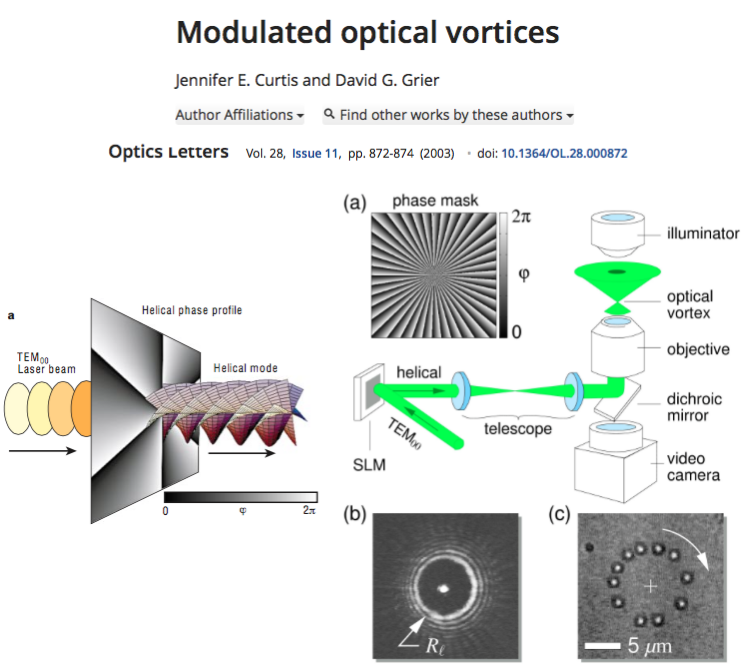
\includegraphics[scale = 0.4]{Figures/presentation/optical_tweezers.pdf}
  \end{figure}
}
\placelogofalse
\frame{
  \frametitle{Aplicaciones de frentes de onda con vorticidad óptica}
  \begin{figure}
    \includegraphics[scale = 0.5]{Figures/presentation/phase_microscopy.png}
  \end{figure}
}
% \frame{
%   \frametitle{Applicaciones de frentes de onda con vorticidad óptica}
%   \begin{figure}
%     \includegraphics[scale = 0.45]{Figures/presentation/spiral_interferometry.png}
%   \end{figure}
% }
\frame{
  \frametitle{Aplicaciones de frentes de onda con vorticidad óptica}
  \begin{figure}
    \includegraphics[scale = 0.5]{Figures/presentation/terabit_com_application.png}
  \end{figure}
}
\placelogotrue

\subsection{Objetivos}
\begin{frame}
  \frametitle{Objetivos planteados en el anteproyecto}
  \begin{block}{Objetivo general}
    Desarrollar la capacidad para generar y caracterizar vórtices de fase
    mediante un modulador espacial de luz (SLM) de transmisión. 
  \end{block}
  \begin{block}{Objetivos espec\'ificos}
    \small
    \begin{enumerate}
	\item Identificar y apropiar los conceptos y
                  procedimientos necesarios para caracterizar
                  moduladores espaciales de luz de transmisión, con
                  miras a la producción y análisis de vórtices
                  ópticos (VOs). 
        \item Implementar una plataforma experimental para
                  caracterizar la modulación de amplitud y fase de un
                  SLM a partir de un montaje interferométrico
                  automatizado. 
         \item Obtener experimentalmente vórtices ópticos del
                  tipo Laguerre-Gauss mediante el uso de un SLM y
                  estudiar las distribuciones de intensidad y fase
                  alrededor de los vórtices. 
         \item Proponer alternativas para el desarrollo de
                  aplicaciones metrológicas basadas en la generación
                  de VOs y el estudio de sus propiedades.
       \end{enumerate}
     \end{block}
   \end{frame}

\section{Generación de vórtices ópticos}
\subsection{Introducción}
\frame{
\frametitle{Vórtices ópticos presentes en haces Laguerre-Gauss}
  \begin{block}{\centering Los haces Laguerre-Gauss son una solución a la ecuación de onda}
   \scriptsize
    \begin{align*}
     u(r,\phi,z) &\propto \frac{z_R}{(z_R^2+z_R^2)}
     \left[\frac{r\sqrt{2}}{w(z)}\right]^lL_p^l\left(\frac{2r^2}{w^2(z)}
     \right)\exp{\left(\frac{-r^2}{w^2(z)}\right)}\nonumber\\
     &\times \exp{\left(\frac{-ikr^2z}{2(z^2+z_R^2)}\right)}
       \highlightG{\exp(-il\phi)}\exp{\left[i\left(2p+l+1\right)\tan^{-1}\frac{z}{z_R}\right]}
     \label{eq:Laguerre-Gauss}
     \end{align*}
  \end{block}
%\pause
\begin{figure}
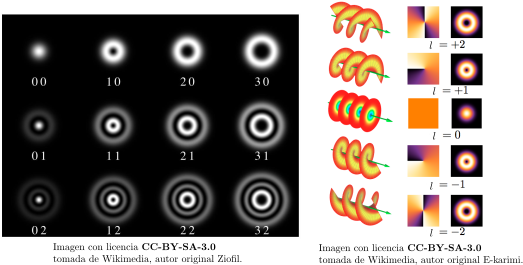
\includegraphics[scale = 0.6]{Figures/presentation/VO_amp_and_phase.pdf}
\end{figure}
}
% \frame{
% \frametitle{Cómo se generan los vórtices ópticos}
% % \begin{columns}
% %   \column{0.3\textwidth}
% %   \begin{figure}
% %     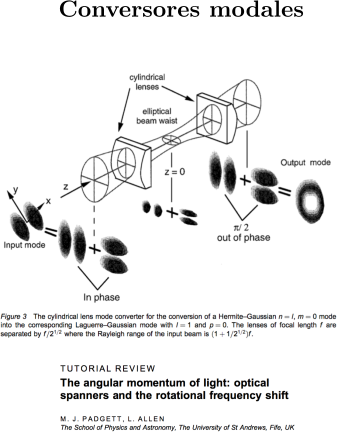
\includegraphics[scale =
% %     0.5]{Figures/presentation/conversores_modales.pdf}
% %   \end{figure}
% %   \pause
% %  \column{0.3\textwidth}
% %   \begin{figure}
% %     \includegraphics[scale =
% %     0.5]{Figures/presentation/spp.pdf}
% %   \end{figure}
% %   \pause
% %   \column{0.4\textwidth}
% %   \begin{figure}
% %     \includegraphics[scale =
% %     0.5]{Figures/presentation/holograms.pdf}
% %   \end{figure}
% % \end{columns}
% \begin{figure}
% \includegraphics[scale=0.39]{Figures/presentation/methods_1.pdf}
% \end{figure}
% }
% \addtocounter{framenumber}{-1}
% \frame{
% \frametitle{Cómo se generan los vórtices ópticos}
% \begin{figure}
% \includegraphics[scale=0.39]{Figures/presentation/methods_2.pdf}
% \end{figure}
% }
% \addtocounter{framenumber}{-1}
\frame{
\frametitle{Cómo se generan los vórtices ópticos}
\begin{figure}
\includegraphics[scale=0.39]{Figures/presentation/methods_3.pdf}
\end{figure}
}
\frame{
\frametitle{Moduladores espaciales de luz}
\begin{figure}
\includegraphics[scale=0.39]{Figures/presentation/SLMs.png}
\end{figure}
%\pause
\begin{figure}
\includegraphics[scale=0.39]{Figures/presentation/SLMs_2.png}
\end{figure}
}
\subsection{Marco teórico}%
\placelogofalse
\frame{
\frametitle{Cristales líquidos del tipo twisted nematic}
\begin{columns}
  \column{0.32\textwidth}
  % \begin{figure}
  %   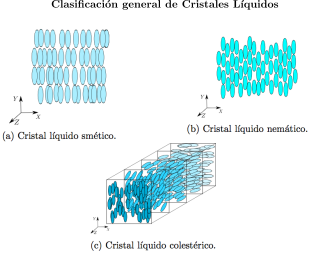
\includegraphics[scale = 0.53]{Figures/presentation/clasificacion_LC.pdf}
  % \end{figure}
  %\pause
  \begin{figure}
    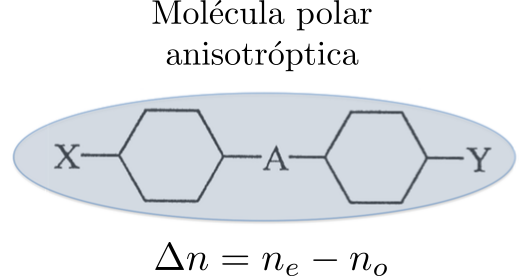
\includegraphics[scale = 0.2]{Figures/presentation/molecula_anisotropica.pdf}
  \end{figure}
  %\pause
  \column{0.6\textwidth}
  \begin{figure}
    \includegraphics[scale = 0.25]{Figures/presentation/TN-LCD.pdf}
  \end{figure}
  \tiny
  \centering
  Tomado de Nestor Uribe-Patarroyo \citep{UribePatarroyo2011} de su
  tesis doctoral con autorizaci\'on. 
\end{columns}
}
\placelogotrue
\frame{
\frametitle{\small El modulador espacial de luz es un sistema que modifica la
  polarización}
  \begin{figure}
    \includegraphics[scale = 0.8]{Figures/presentation/polarization_system_1.pdf}
  \end{figure}
}
\addtocounter{framenumber}{-1}
\frame{
\frametitle{\small El modulador espacial de luz es un sistema que modifica la
  polarización}
  \begin{figure}
    \includegraphics[scale = 0.8]{Figures/presentation/polarization_system_2.pdf}
  \end{figure}
}
\addtocounter{framenumber}{-1}
\frame{
\frametitle{\small El modulador espacial de luz es un sistema que modifica la
  polarización}
  \begin{figure}
    \includegraphics[scale = 0.8]{Figures/presentation/polarization_system_2d5.pdf}
  \end{figure}
}
\addtocounter{framenumber}{-1}
% \frame{
% \frametitle{\small El modulador espacial de luz es un sistema que modifica la
%   polarización}
%   \begin{figure}
%     \includegraphics[scale = 0.8]{Figures/presentation/polarization_system_3.pdf}
%   \end{figure}
% }
\addtocounter{framenumber}{-1}
% \frame{
% \frametitle{\small El modulador espacial de luz es un sistema que modifica la
%   polarización}
%   \begin{figure}
%     \includegraphics[scale = 0.8]{Figures/presentation/polarization_system_4.pdf}
%   \end{figure}
% }
% \addtocounter{framenumber}{-1}
\frame{
\frametitle{\small El modulador espacial de luz es un sistema que modifica la
  polarización}
  \begin{figure}
    \includegraphics[scale = 0.8]{Figures/presentation/polarization_system_4d5.pdf}
  \end{figure}
}
% \frame{
% \frametitle{\small El modulador espacial de luz es un sistema que modifica la
%   polarización}
%   \begin{figure}
%     \includegraphics[scale = 0.8]{Figures/presentation/polarization_system_5.pdf}
%   \end{figure}
% }
% \addtocounter{framenumber}{-1}
% \frame{
% \frametitle{\small El modulador espacial de luz es un sistema que modifica la
%   polarización}
%   \begin{figure}
%     \includegraphics[scale = 0.8]{Figures/presentation/polarization_system_6.pdf}
%   \end{figure}
% }
\addtocounter{framenumber}{-1}
\subsection{Caracterización de un modulador espacial de luz de transmisión}
\subsubsection{Caracterización de la modulación de amplitud}
\frame{
   \frametitle{Contenido}
   \footnotesize 
   \tableofcontents[currentsubsection]%,hideothersubsections]
}
% \frame{
% \frametitle{Medida de la modulación de amplitud del SLM}
%   \begin{figure}
%     \includegraphics[scale = 0.5]{Figures/presentation/amplitude_measure_1.pdf}
%   \end{figure}
% }
% \addtocounter{framenumber}{-1}
% \frame{
% \frametitle{Medida de la modulación de amplitud del SLM}
%   \begin{figure}
%     \includegraphics[scale = 0.5]{Figures/presentation/amplitude_measure_2.pdf}
%   \end{figure}
% }
% \addtocounter{framenumber}{-1}
\frame{
\frametitle{Medida de la modulación de amplitud del SLM}
  \begin{figure}
    \includegraphics[scale = 0.5]{Figures/presentation/amplitude_measure_ZIP.pdf}
  \end{figure}
}
\addtocounter{framenumber}{-1}
% \frame{
% \frametitle{Medida de la modulación de amplitud del SLM}
%   \begin{figure}
%     \includegraphics[scale = 0.5]{Figures/presentation/amplitude_measure_5.pdf}
%   \end{figure}
% }
% \addtocounter{framenumber}{-1}
% \frame{
% \frametitle{Medida de la modulación de amplitud del SLM}
%   \begin{figure}
%     \includegraphics[scale = 0.5]{Figures/presentation/amplitude_measure_6.pdf}
%   \end{figure}
% }
\addtocounter{framenumber}{-1}
\frame{
\frametitle{Medida de la modulación de amplitud del SLM}
  \begin{figure}
    \includegraphics[scale = 0.5]{Figures/presentation/amplitude_measure_3.pdf}
  \end{figure}
}

% \frame{
% \frametitle{El método de Ma et al.~ para la caracterización del SLM}
%   \begin{figure}
%     \includegraphics[scale = 0.5]{Figures/presentation/Ma_method_1.pdf}
%   \end{figure}
% }
% \addtocounter{framenumber}{-1}
% \frame{
% \frametitle{El método de Ma et al.~ para la caracterización del SLM}
%   \begin{figure}
%     \includegraphics[scale = 0.5]{Figures/presentation/Ma_method_2.pdf}
%   \end{figure}
% }
%\addtocounter{framenumber}{-1}
\frame{
\frametitle{El método de Ma et al.~ para la caracterización del SLM}
  \begin{figure}
    \includegraphics[scale = 0.5]{Figures/presentation/Ma_method_3.pdf}
  \end{figure}
}
\addtocounter{framenumber}{-1}
% \frame{
% \frametitle{El método de Ma et al.~ para la caracterización del SLM}
%   \begin{figure}
%     \includegraphics[scale = 0.5]{Figures/presentation/Ma_method_4.pdf}
%   \end{figure}
% }
% \addtocounter{framenumber}{-1}
\frame{
\frametitle{El método de Ma et al.~ para la caracterización del SLM}
  \begin{figure}
    \includegraphics[scale = 0.5]{Figures/presentation/Ma_method_5.pdf}
  \end{figure}
}
\addtocounter{framenumber}{-1}
\frame{
\frametitle{El método de Ma et al.~ para la caracterización del SLM}
  \begin{figure}
    \includegraphics[scale = 0.5]{Figures/presentation/Ma_method_6.pdf}
  \end{figure}
}
\frame{
\frametitle{Comprobación experimental con 100 medidas}
  \begin{figure}
    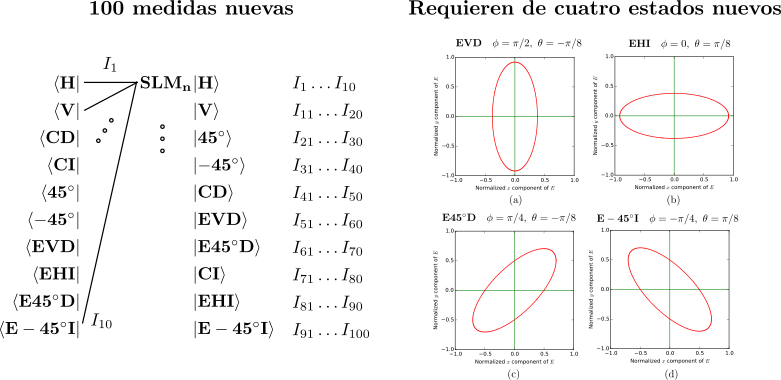
\includegraphics[scale = 0.56]{Figures/presentation/100_measures.pdf}
  \end{figure}
}
\frame{
  \frametitle{\small Resultados de la caracterización de amplitud con el método
de Ma et~al.}
  \begin{figure}
    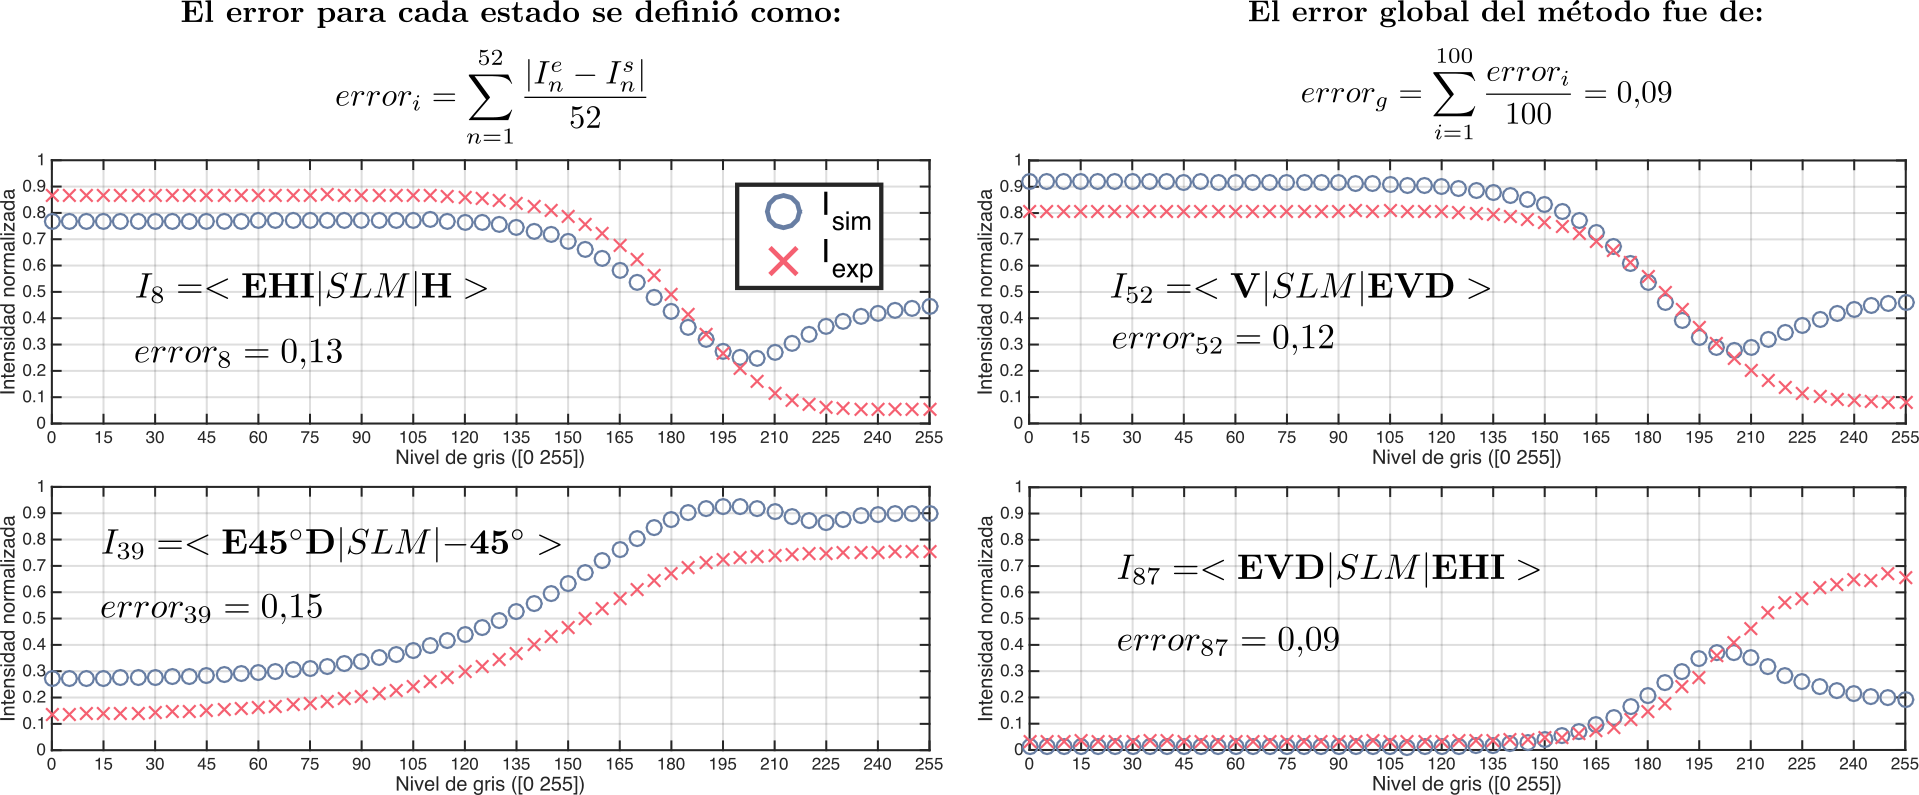
\includegraphics[scale = 0.225]{Figures/presentation/Ma_results.pdf}
  \end{figure}
}
\frame{
\frametitle{\small Un método nuevo basado en minimización de parámetros}
  \begin{figure}
    \includegraphics[scale = 0.6]{Figures/presentation/our_method_1.pdf}
  \end{figure}
}
\addtocounter{framenumber}{-1}
\frame{
\frametitle{\small Un método nuevo basado en minimización de parámetros}
  \begin{figure}
    \includegraphics[scale = 0.6]{Figures/presentation/our_method_2.pdf}
  \end{figure}
}
\frame{
  \frametitle{\small Resultados de la caracterización de amplitud con el método
de minimizaci\'on}
  \begin{figure}
    \includegraphics[scale = 0.65]{Figures/presentation/Min_results.pdf}
  \end{figure}
}
% \frame{
% \frametitle{Ampliaci\'on del nuevo método}
%   \begin{figure}
%     \includegraphics[scale = 0.5]{Figures/presentation/Min_100_results_1.pdf}
%   \end{figure}
% }
% \addtocounter{framenumber}{-1}
\frame{
\frametitle{Ampliaci\'on del nuevo método}
  \begin{figure}
    \includegraphics[scale = 0.5]{Figures/presentation/Min_100_results_2.pdf}
  \end{figure}
}
%\addtocounter{framenumber}{-1}
\frame{
\frametitle{Resultados de la caracterizaci\'on con 100 medidas}
  \begin{figure}
    \includegraphics[scale = 0.68]{Figures/presentation/Min_100_results_3.pdf}
  \end{figure}
}
% \frame{
% \frametitle{Una plataforma para la automatización de medidas}
%   \begin{figure}
%     \includegraphics[scale = 0.7]{Figures/presentation/montaje_experimental_amp_1.pdf}
%   \end{figure}
% }
% \addtocounter{framenumber}{-1}
% \frame{
% \frametitle{Una plataforma para la automatización de medidas}
%   \begin{figure}
%     \includegraphics[scale = 0.7]{Figures/presentation/montaje_experimental_amp_4.pdf}
%   \end{figure}
% }
% \addtocounter{framenumber}{-1}
\frame{
\frametitle{Una plataforma para la automatización de medidas}
  \begin{figure}
    \includegraphics[scale = 0.7]{Figures/presentation/montaje_experimental_amp_3.pdf}
  \end{figure}
}
\addtocounter{framenumber}{-1}
\frame{
\frametitle{Una plataforma para la automatización de medidas}
  \begin{figure}
    \includegraphics[scale = 0.9]{Figures/presentation/plataforma_digital_1.pdf}
  \end{figure}
}
\addtocounter{framenumber}{-1}
\frame{
\frametitle{Una plataforma para la automatización de medidas}
  \begin{figure}
    \includegraphics[scale = 0.9]{Figures/presentation/plataforma_digital_2.pdf}
  \end{figure}
}
% \addtocounter{framenumber}{-1}
% \frame{
% \frametitle{Una plataforma para la automatización de medidas}
%   \begin{figure}
%     \includegraphics[scale = 0.9]{Figures/presentation/plataforma_digital_3.pdf}
%   \end{figure}
% }
\subsubsection{Caracterización de la modulación de fase}
\frame{
   \frametitle{Contenido}
   \footnotesize 
   \tableofcontents[currentsubsection]%,hideothersubsections]
}
% \frame{
% \frametitle{Medida de la modulaci\'on de fase}
%   \begin{figure}
%     \includegraphics[scale = 0.54]{Figures/presentation/medida_fase_1.pdf}
%   \end{figure}
% }
% \addtocounter{framenumber}{-1}
\frame{
\frametitle{Medida de la modulaci\'on de fase}
  \begin{figure}
    \includegraphics[scale = 0.54]{Figures/presentation/medida_fase_2.pdf}
  \end{figure}
}
\addtocounter{framenumber}{-1}
\frame{
\frametitle{Medida de la modulaci\'on de fase}
  \begin{figure}
    \includegraphics[scale = 0.54]{Figures/presentation/medida_fase_3.pdf}
  \end{figure}
}
\addtocounter{framenumber}{-1}
\frame{
\frametitle{Medida de la modulaci\'on de fase}
  \begin{figure}
    \includegraphics[scale = 0.54]{Figures/presentation/medida_fase_4.pdf}
  \end{figure}
}
\frame{
\frametitle{Algunos estados representativos del SLM}
  \begin{figure}
    \includegraphics[scale = 0.3]{Figures/presentation/phase_results_1.pdf}
  \end{figure}
}
\frame{
\frametitle{El mejor estado encontrado}
  \begin{figure}
    \includegraphics[scale = 0.4]{Figures/presentation/phase_results_2.pdf}
  \end{figure}
}

\subsection{Resultados experimentales}
\frame{
   \frametitle{Contenido}
   \footnotesize 
   \tableofcontents[currentsubsection]%,hideothersubsections]
}
\placelogofalse
\frame{
\frametitle{Una plataforma para la generación de máscaras de fase}
\begin{figure}
\includegraphics[scale=0.3]{Figures/ch2_img/mask_app.png}
\end{figure}
}
\placelogotrue
\frame{
 \frametitle{Resultados experimentales: Generación de VOs en eje}
\begin{figure}
  \includegraphics[scale = 0.2]{Figures/ch2_img/OV_I10.pdf}
\end{figure}
% \pause
\begin{figure}
  \includegraphics[scale = 0.2]{Figures/ch2_img/OV_I6.pdf}
\end{figure}
}
\frame{
 \frametitle{\small Resultados experimentales: Generación de VOs fuera de
   eje}
\begin{figure}
  \includegraphics[scale=.5]{Figures/ch2_img/fork_recipe.pdf}
\end{figure}
}
\frame{
 \frametitle{\small Resultados experimentales: Generación de VOs fuera de
   eje}
\begin{figure}
  \includegraphics[scale = 0.23]{Figures/ch2_img/diffracted_OV_I6_and_I10.pdf}
\end{figure}
}
\frame{
 \frametitle{\small Resultados experimentales: Generación de VOs fuera de
   eje}
\begin{figure}
  \includegraphics[scale = 0.23]{Figures/ch2_img/diffracted_OV_I6_and_I10_2.pdf}
\end{figure}
}
\addtocounter{framenumber}{-1}
\section{Caracterización de aberraciones de vórtices ópticos}
\subsection{Introducción}
\frame{
  \frametitle{Fuentes de aberraciones}
\begin{columns}[t]
\small
\column{0.5 \textwidth}
Pueden deberse a imperfecciones en:
\begin{itemize}
  \item el diseño,
  \item los materiales,
  \item la manufactura,
 \item o la alineación 
\end{itemize}
de elementos ópticos.
\vspace{0.5cm}

En nuestro caso, se deben también a los efectos no deseados que introducen algunas
características del SLM como las distintas formas de discretización, el
acople entre modulación de fase y de amplitud y el factor de llenado.
\column{0.5 \textwidth}
\begin{figure}
  \includegraphics[scale = .28]{Figures/presentation/discrete_mask2.png}
\end{figure}
% \begin{figure}
% \includegraphics[scale =.5]{Figures/presentation/fill_factor.jpg}
% \caption{}
% \end{figure}
\end{columns}
}
\frame{
\frametitle{¿Cómo caracterizar las aberraciones?}
\begin{figure}
\includegraphics[scale = .9]{Figures/presentation/retrieval_methods_1.pdf}
\end{figure}
}
\addtocounter{framenumber}{-1}
\frame{
\frametitle{¿Cómo caracterizar las aberraciones?}
\begin{figure}
\includegraphics[scale = .9]{Figures/presentation/retrieval_methods.pdf}
\end{figure}
}
\subsection{Marco teórico}
\frame[t]{
\frametitle{Marco teórico: Sistemas formadores de imagen}
\begin{columns}
  \column{0.5\textwidth}
\scriptsize
\justifying
Las t\'ecnicas de phase retrieval analizan el efecto de las
aberraciones sobre las imágenes que produce un sistema \'optico. 
Las aberraciones son caracterizadas cuando se encuentra una funci\'on de transferencia que reproduce las
im\'agenes registradas. 
\column{0.5\textwidth}
\begin{figure}
    \includegraphics[scale =.4]{Figures/presentation/sistema.pdf}
  \end{figure}
\end{columns}
\vspace{-0.5cm}
\begin{columns}
  % \pause
  \column{0.3\textwidth}
  % \begin{block}{Transformaciones en sistemas no coherentes}
  %     \begin{equation}\label{eq:Output_Image}
  %       d(\vec{x}) = d_{obj}(\vec{x}) \otimes s(\vec{x}).
  %     \end{equation}
  %     \begin{equation}\label{eq:Output_Image_fourier}
  %     D(\vec{u}) = D_{obj}(\vec{u})S(\vec{u}).
  %     \end{equation}
  % \end{block}
  % \begin{block}{Transformaciones en sistemas coherentes}
  %   \begin{equation}\label{eq:Output_Image_complex}
  %     u(\vec{x}) = u_{obj}(\vec{x}) \otimes h(\vec{x}).
  %   \end{equation}
  %   \begin{equation}\label{eq:Output_F_Image_complex}
  %     U(\vec{u}) = U_{obj}(\vec{u})H(\vec{u}).
  %   \end{equation}
  % \end{block}
  \begin{figure}
    \includegraphics[scale =.88]{Figures/presentation/transformations.pdf}
  \end{figure}
  \pause
 \column{0.3\textwidth}
  \begin{figure}
    \includegraphics[scale =.85]{Figures/presentation/definitions.pdf}
  \end{figure}
  % \pause
 \column{0.3\textwidth}
  \begin{figure}
    \includegraphics[scale =.85]{Figures/presentation/relations.pdf}
  \end{figure}
\end{columns}
% \begin{columns}
%   \column{0.5\textwidth}
%  Introducir una fase al sistema implica añadir un bloque nuevo a la
%  función de transferencia.  
% \end{columns} ñ
}
\frame{
\frametitle{Marco teórico: Phase diversity }
\small
\begin{columns}
  \column{0.7\textwidth}
   \begin{figure}
     \includegraphics[scale=.3]{Figures/presentation/sistema_PD.pdf}
   \end{figure}
   % \pause
   \begin{figure}
     \includegraphics[scale=.3]{Figures/presentation/sistema_PD_2.pdf}
   \end{figure}
% \pause
  \column{0.3\textwidth}
   \begin{figure}
     \includegraphics[scale=.4]{Figures/presentation/diversities.pdf}
   \end{figure}
\end{columns}
\pause
\begin{block}{\centering Funcional de minimizaci\'on}
   \begin{equation*}\label{eq:metric}
   L(\bar{D}_{obj}, \phi)= \sum_{j=0}^{K} \sum_{u,v}^{M,N}  \left |D_{j} - \bar{D}_{obj} S_{j} \right | ^2.
   \end{equation*} 
\end{block}
}
\frame{
\frametitle{\small Marco teórico: Phase diversity con iluminaci\'on
  coherente}
\begin{columns}
  \column{0.5\textwidth}
    \begin{figure}
      \includegraphics[scale = 0.7]{Figures/presentation/our_PD.pdf}
    \end{figure}
   \pause
  \column{0.5\textwidth}
    \begin{figure}[t]
      \includegraphics[scale = 0.6]{Figures/presentation/our_PD_right.pdf}
    \end{figure}
\end{columns}
% \pause
\begin{block}{\centering Un nuevo funcional de minimizaci\'on}
\begin{equation*}
L_j(\phi)= \sum_{j=0}^{K} \sum_{u,v}^{M,N}  \left |d_{j} - |u_j|^2
\right | ^2
\label{eq:metric_coherent}
\end{equation*}
\end{block}
}
\frame{
\frametitle{\small Marco teórico: Phase diversity con iluminaci\'on coherente mejorado
  con VOs}
\begin{columns}
  \column{0.4\textwidth}
  \begin{block}{\footnotesize Una nueva familia de diversidades}
\footnotesize
    $$\psi_l = arg(\exp{(il \theta)}),$$
    \begin{equation*}\label{eq:newGP}
      u_j^l =  \mathcal{F}^{- 1}\{U_{obj} A e^{i\left(
          \phi+ \psi_l + \phi_j \right)} \}.
    \end{equation*}
  \end{block}
  % \pause
  \column{0.5\textwidth}
  \begin{block}{\centering \footnotesize Funcional extendido}
\footnotesize
    \begin{equation}\label{eq:metric_coherent_OAMs}
      L(\phi)= \sum_{l=0}^L\sum_{j=0}^{K} \sum_{u,v}^{M,N}  \left |d_{j}^l - |u_j^l|^2 \right | ^2.
    \end{equation}
  \end{block}
\end{columns}
% \pause
  \begin{figure}
   \includegraphics[scale = 0.8]{Figures/presentation/montaje_dibujo.pdf}
  \end{figure}
}

\frame{
\frametitle{Marco teórico: Algoritmo de la implementaci\'on}
\begin{figure}
  \includegraphics[scale = .85]{Figures/chPD_img/PDLightFlux_simple_esp.pdf}
\end{figure}
}
\subsection{Aberraciones simuladas}
\frame{
\frametitle{Detección de aberraciones simuladas: Metodología}
\begin{figure}
\includegraphics[scale = 0.65]{Figures/presentation/simulation_methodology_1.pdf}
\end{figure}
%http://all-free-download.com/free-vector/download/two_red_dice_clip_art_12898.html
%Dice image
}
\addtocounter{framenumber}{-1}
\frame{
\frametitle{Detección de aberraciones simuladas: Metodología}
\begin{figure}
\includegraphics[scale = 0.65]{Figures/presentation/simulation_methodology_2.pdf}
\end{figure}
}
\addtocounter{framenumber}{-1}
\frame{
\frametitle{Detección de aberraciones simuladas: Metodología}
\begin{figure}
\includegraphics[scale = 0.65]{Figures/presentation/simulation_methodology_3.pdf}
\end{figure}
}
\frame{
\frametitle{Detección de aberraciones simuladas: Resultados}
\begin{figure}
  \includegraphics[scale = .4]{Figures/chPD_img/mixed_wf_errors_esp.pdf}
\end{figure}
}
\addtocounter{framenumber}{-1}
\frame{
\frametitle{Detección de aberraciones simuladas: Resultados}
\begin{figure}
  \includegraphics[scale = .25]{Figures/chPD_img/phase_comparison_esp.pdf}
\end{figure}
}
\addtocounter{framenumber}{-1}
\frame{
\frametitle{Detección de aberraciones simuladas: Resultados}
\begin{figure}
  \includegraphics[scale = .2]{Figures/chPD_img/phase_comparison_esp_2.pdf}
\end{figure}
}
\subsection{Aberraciones experimentales}
\frame{
   \frametitle{Contenido}
   \footnotesize 
   \tableofcontents[currentsubsection]%,hideothersubsections]
}
\frame{
\frametitle{Detección de aberraciones experimentales: Metodología}
\begin{figure}
\includegraphics[scale = 0.7]{Figures/presentation/montaje.pdf}
\end{figure}
}
\frame{
\frametitle{Detección de aberraciones experimentales: Metodología}
\begin{figure}
\includegraphics[scale = 0.4]{Figures/presentation/exp_methodology.pdf}
\end{figure}
}
\frame{
\frametitle{Detección de aberraciones experimentales: Resultados}
\begin{figure}
\includegraphics[scale = 0.7]{Figures/chPD_img/experimental_results_correction.pdf}
\end{figure}
}
\frame{
\frametitle{Detección de aberraciones experimentales: Resultados}
\begin{figure}
\includegraphics[scale = 0.7]{Figures/presentation/exp_res_correction_1.pdf}
\end{figure}
}
% \addtocounter{framenumber}{-1}
% \frame{
% \frametitle{Detección de aberraciones experimentales: Resultados}
% \begin{figure}
% \includegraphics[scale = 0.7]{Figures/presentation/exp_res_correction_2.pdf}
% \end{figure}
% }
\subsection{Propuesta de una aplicación para metrología}
\frame{
\frametitle{Propuesta de una aplicación para metrología}
\begin{figure}
\includegraphics[scale = 0.55]{Figures/presentation/propuesta_1.pdf}
\end{figure}
}
\frame{
\frametitle{Propuesta de una aplicación para metrología}
\begin{figure}
\includegraphics[scale = 0.55]{Figures/presentation/propuesta_2.pdf}
\end{figure}
}
\addtocounter{framenumber}{-1}
\section{Conclusiones y trabajo futuro}	
\begin{frame}{Conclusiones I}
\small
\begin{itemize}
  \item Se mostró el resultado de una labor investigativa con la cual
    fue posible establecer un marco y teórico y una metodología para la
    caracterización y puesta a punto de un TN-SLM. 
 \pause
 \item  Se presentó un sistema automatizado para la caracterización de 
   elementos birrefringentes que se compone de una parte física, y una parte de
    software. 
 \pause
 \item  Asimismo, se desarrolló y puso en proceso de registro una aplicacion de software en la
    plataforma Matlab$\circledR$ para la
    generación de máscaras de fase arbitrarias a ser proyectadas en el
    SLM. Esta aplicación permite:
    \begin{itemize}
      \item Crear máscaras de fase espiral de carga entera arbitraria
        sumadas a:
        \begin{itemize}
          \item Lentes.
          \item Rejillas de difracción de varios tipos.
          \item Aberraciones ópticas compuestas a partir de polinomios
            de Zernike.
        \end{itemize}
      \item Discretizar las máscaras de fase en la cantidad de niveles
        deseados, y asignando valores predeterminados a cada uno. 
\end{itemize}
% \item Por otra parte, se propuso un método novedoso para la
%   caracterización de SLMs basado en el análisis de desplazamiento de
%   franjas en un interferómetro con brazos que no comparten el mismo
%   estado de polarización. Este método ha sido demostrado en
%   simulaciones y nos encontramos en el proceso de corroboración
%   experimental para validarlo. 
\pause
\item  Se generaron VOs en un sistema óptico 4F usando dos tipos distintos de
   máscaras de fase. Y se detectó que aún con buena modulación no se
   corrigen del todo las aberraciones.  
\pause
\end{itemize}
\end{frame}

\begin{frame}{Conclusiones II}
\small
\begin{itemize}
\item Se desarrolló un método traído de aplicaciones
  en astronomía para la detección y corrección de aberraciones ópticas
  en haces con vorticidad óptica.
\pause
\item Este método fue validado mediante numerosas simulaciones, y
  experimentos y se propuso como la base para un instrumento que puede
  ser usado en aplicaciones metrológicas. 
\end{itemize}
\end{frame}

\begin{frame}
  \frametitle{Trabajo futuro}
\begin{itemize}
  \item Estudiar la generación de vórtices ópticos con iluminación
    parcialmente coherente y
 \pause
 \item extender el método de PD para este caso.
 \pause
  \item Exploración de una técnica de polarimetría-interfermoétrica
    basada en derivada de las investigaciones para la caracterización
    del SLM.
 \pause
 \item Implementar la propuesta de una herramienta basada en nuestro
   método para la caracterización de sistemas complejos. Por ejemplo
   sistemas de escritura punto a punto en hologramas sintéticos.
 \pause
 \item Aplicar los métodos y habilidades desarrollados para la
   implementación de un microscopio de fase con iluminación espiral.
\end{itemize}
\end{frame}
\begin{frame}{¿Preguntas?}
  \begin{figure}
    \centering
    \includegraphics[scale=0.5]{Figures/presentation/thinker.jpeg}	
  \end{figure}
\end{frame}
\placelogofalse
\section{Bibliografía}
\tiny
  \begin{frame}[allowframebreaks]
  \frametitle{Bibliograf\'ia}
\nocite{*}
  \bibliographystyle{unsrt}
  \bibliography{References/presentation_references}
  \end{frame}
\placelogotrue
%\subsection{Contexto}
   
 \begin{frame}
   \frametitle{Contexto}
   \begin{block}{\centering Proyecto interinstitucional en curso} 
	\justifying
   Aberraciones ópticas en haces Laguerre-Gaussianos:
       corrección y aplicaciones metrológicas; 2013 – 2015
   \end{block}
   \begin{figure}
     \centering
     \includegraphics[scale = .5]{Figures/presentation/instituciones.png}
   \end{figure}
 \end{frame}
 
 \begin{frame}
   \frametitle{Contexto}
   \begin{figure}
     \centering
     \includegraphics[scale = .5]{Figures/presentation/jovenes_inv_conv.png}
   \end{figure}
 \end{frame}
 \begin{frame}
   \frametitle{Contexto}
   \begin{figure}
     \centering
     \includegraphics[scale = .5]{Figures/presentation/inta_conv.png}
   \end{figure}
 \end{frame}
\frame{
\frametitle{Método Gerbercht-Saxton}
\begin{figure}
\includegraphics[scale = 0.28]{Figures/chPD_img/GS_algorithm.pdf}
\end{figure}
}
\end{document}
